\documentclass[10pt,twocolumn,letterpaper]{article}

% --- Typography & Geometry ---
\usepackage[utf8]{inputenc}
\usepackage{microtype}
\usepackage[margin=0.75in,top=0.85in,bottom=0.85in]{geometry}

% --- Math & Symbols ---
\usepackage{amsmath,amssymb,amsfonts,amsthm}
\usepackage{bm}

% --- Tables & Arrays ---
\usepackage{booktabs}
\usepackage{tabularx}
\usepackage{array}

% --- Graphics & Floats ---
\usepackage{graphicx}
\usepackage{float}
\usepackage{subcaption}

% --- Code Listings ---
\usepackage{xcolor}
\usepackage{listings}

\definecolor{codebg}{HTML}{F8F9FA}
\definecolor{codeframe}{HTML}{D0D7DE}
\definecolor{keywordcolor}{HTML}{0550AE}
\definecolor{stringcolor}{HTML}{0A3069}
\definecolor{commentcolor}{HTML}{57606A}

\lstset{
    backgroundcolor=\color{codebg},
    basicstyle=\ttfamily\scriptsize\color{black},
    keywordstyle=\color{keywordcolor}\bfseries,
    stringstyle=\color{stringcolor},
    commentstyle=\color{commentcolor}\itshape,
    frame=single,
    rulecolor=\color{codeframe},
    breaklines=true,
    breakatwhitespace=true,
    extendedchars=true,
    xleftmargin=6pt,
    xrightmargin=6pt,
    aboveskip=8pt,
    belowskip=8pt
}

% --- Hyperlinks ---
\usepackage{hyperref}
\hypersetup{
    colorlinks=true,
    linkcolor=blue!70!black,
    citecolor=blue!70!black,
    urlcolor=blue!70!black
}

% --- Input Title & Authors ---

\section{GQA: Grouped-Query Attention for Memory-Efficient Transformer Inference}


\textbf{Authors:}
\begin{itemize}
\item {{AUTHOR\_1\_NAME}}  -- {{AUTHOR\_1\_EMAIL}}
\end{itemize}
\begin{itemize}
\item {{AUTHOR\_2\_NAME}}  -- {{AUTHOR\_2\_EMAIL}}
\end{itemize}

\textbf{Affiliations:}
\begin{itemize}
\item   {{UNIVERSITY\_1}}, {{DEPARTMENT\_1}}
\end{itemize}
\begin{itemize}
\item   {{UNIVERSITY\_2}}, {{DEPARTMENT\_2}}
\end{itemize}

\textbf{Corresponding author:} {{CORRESPONDING\_AUTHOR}}
\textbf{Preprint date:} {{DATE}}
\textbf{Version:} v{{VERSION}}
\textbf{Code:} https://github.com/{{ORG}}/SVD\_Project/tree/main/framework/attentions/gqa.py
\textbf{Model weights:} https://huggingface.co/{{HF\_ORG}}
\textbf{License:} {{LICENSE}}



\subsection{Abstract}

Autoregressive transformer inference is bottlenecked by the memory footprint of 
the key-value (KV) cache, which scales linearly with sequence length and number 
of heads. Multi-Head Attention (MHA) stores one $K$ and $V$ per query head 
($H_{KV} = H$), which is maximally expressive but also maximally memory-intensive. 
Multi-Query Attention (MQA) collapses all KV heads into one ($H_{KV} = 1$), 
achieving minimal memory at a cost to quality. \textbf{Grouped-Query Attention} (GQA) 
interpolates between these extremes: it partitions the $H$ query heads into $G$ 
groups and shares a single KV head per group ($H_{KV} = G \le H$).

We present a production-hardened PyTorch implementation of GQA that supports 
flat (DistilBERT), nested (RoBERTa), causal (GPT-2), and grouped-query (Qwen3.5) 
architectures. Our implementation includes exact pretrained weight transfer 
via \texttt{copy\\_weights}, frozen base weights with LoRA recovery adapters, RoPE 
support, and safe injection returning \texttt{None} on failure. We evaluate GQA on 
DistilBERT, RoBERTa-base, and GPT-2 on SST-2 with $G = H/2$ (i.e., 
$H_{KV} = {{KV_HEADS}}$), achieving \textbf{{{D\_ACC}}\%}, \textbf{{{R\_ACC}}\%}, and 
\textbf{{{G\_ACC}}\%} accuracy respectively. The KV cache footprint is reduced by 
\textbf{{{KV\_REDUCTION}}$\times$} at inference time. We provide a full ablation over 
$G / H$ ratio and analyze the trade-off between memory savings and quality loss.

\textbf{Keywords:} grouped-query attention, KV cache, memory efficiency, transformer 
inference, attention architecture



\subsection{Lay Summary}

When a chatbot generates text, it needs to remember the previous tokens it 
has seen. This "memory" is called the KV cache, and it grows linearly with 
the length of the conversation. For long conversations, this memory can 
become the bottleneck -- not the model's weights, but the activations it 
stores per token.

GQA solves this by sharing memory between groups of attention heads. Instead 
of storing a separate memory per head (as MHA does) or a single shared memory 
for all heads (as MQA does), it stores one memory per group of heads. This 
gives a smooth trade-off: fewer groups means less memory but slightly lower 
quality.

Our implementation supports four popular architectures and includes 
production-hardened features like fallback on failure and exact weight 
transfer from pretrained models. On three benchmark models, GQA achieves 
near-baseline accuracy while cutting KV cache memory by ~2$\times$.



\subsection{Table of Contents}

1. [Introduction](01\_intro.md)
2. [Related Work](02\_related.md)
3. [Background](03\_background.md)
4. [Method](04\_method.md)
5. [Architecture Integration](05\_architecture.md)
6. [Experimental Setup](06\_setup.md)
7. [Results](07\_results.md)
8. [Analysis](08\_analysis.md)
9. [Discussion](09\_discussion.md)
10. [Limitations](10\_limitations.md)
11. [Conclusion](11\_conclusion.md)
12. [Reproducibility](12\_reproducibility.md)
13. [References](13\_references.md)

\textbf{Appendices:}
\begin{itemize}
\item [A. Mathematical Derivations](A\_math.md)
\end{itemize}
\begin{itemize}
\item [B. Implementation Details](B\_implementation.md)
\end{itemize}
\begin{itemize}
\item [C. Full Experimental Data](C\_data.md)
\end{itemize}
\begin{itemize}
\item [D. Negative Results](D\_negative\_results.md)
\end{itemize}
\begin{itemize}
\item [E. Ethical Considerations](E\_ethics.md)
\end{itemize}

\begin{document}

\maketitle

% --- Abstract & Keywords Block ---
\begin{abstract}
Autoregressive transformer inference is bottlenecked by the memory footprint of 
the key-value (KV) cache, which scales linearly with sequence length and number 
of heads. Multi-Head Attention (MHA) stores one $K$ and $V$ per query head 
($H_{KV} = H$), which is maximally expressive but also maximally memory-intensive. 
Multi-Query Attention (MQA) collapses all KV heads into one ($H_{KV} = 1$), 
achieving minimal memory at a cost to quality. **Grouped-Query Attention** (GQA) 
interpolates between these extremes: it partitions the $H$ query heads into $G$ 
groups and shares a single KV head per group ($H_{KV} = G \le H$).

We present a production-hardened PyTorch implementation of GQA that supports 
flat (DistilBERT), nested (RoBERTa), causal (GPT-2), and grouped-query (Qwen3.5) 
architectures. Our implementation includes exact pretrained weight transfer 
via `copy\_weights`, frozen base weights with LoRA recovery adapters, RoPE 
support, and safe injection returning `None` on failure. We evaluate GQA on 
DistilBERT, RoBERTa-base, and GPT-2 on SST-2 with $G = H/2$ (i.e., 
$H_{KV} = 6$), achieving **88.5\%**, **75.5\%**, and 
**77.0\%** accuracy respectively. The KV cache footprint is reduced by 
**{{KV\_REDUCTION}}$\times$** at inference time. We provide a full ablation over 
$G / H$ ratio and analyze the trade-off between memory savings and quality loss.

**Keywords:** grouped-query attention, KV cache, memory efficiency, transformer 
inference, attention architecture

---

\vspace{0.5em}
\noindent\textbf{Keywords:} grouped-query attention, KV cache, memory efficiency, transformer
\end{abstract}

\vspace{1em}

% --- Paper Body ---

\section{1. Introduction}

\subsection{1.1 Motivation}

Autoregressive inference in transformer models is memory-bound, not 
compute-bound. During generation, the model stores keys and values for every 
past token in a \textbf{KV cache}, whose size is:

\[
\text{KV size} = 2 \cdot H_{KV} \cdot d_h \cdot L \cdot B \cdot \text{bytes}
\tag{1.1}
\]

where $H_{KV}$ is the number of KV heads, $d_h$ is the per-head dimension, 
$L$ is the sequence length, and $B$ is the batch size. For a 12-layer GPT-2 
model with $H = 12$, $d_h = 64$, $L = 1024$, and $B = 1$, the KV cache at 
FP16 is:

\[
2 \cdot 12 \cdot 64 \cdot 1024 \cdot 12 \cdot 2 = 37.7 \text{ MB}
\tag{1.2}
\]

which is \textbf{5\% of the model's 774 MB weight footprint} -- small in isolation, 
but growing linearly with sequence length and batch size. At $L = 32{,}768$ 
and $B = 8$, the KV cache dominates inference memory, requiring \textbf{9.6 GB} 
per layer group, exceeding most consumer GPUs.

Two extremes have been explored to reduce this cost:

1. \textbf{Multi-Head Attention (MHA).} Each of the $H$ query heads has its own 
   $K$ and $V$ ($H_{KV} = H$). Maximally expressive, maximally memory-intensive.
2. \textbf{Multi-Query Attention (MQA).} All query heads share a single $K, V$ 
   pair ($H_{KV} = 1$). Minimal memory, but empirically worse quality, 
   especially on tasks requiring fine-grained attention.

\textbf{Grouped-Query Attention (GQA)} was introduced as a middle ground: partition 
the $H$ query heads into $G$ groups, each with a dedicated $K, V$ pair 
($H_{KV} = G$). The KV cache shrinks by a factor of $H / G$, and quality 
degrades gracefully with $G$.

\subsection{1.2 Problem Statement}

Given a pretrained MHA-based model $\mathcal{M}$ with $H$ query heads and 
$H_{KV} = H$, we seek a modified model $\mathcal{M}'$ such that:

\[
\mathcal{M}' \approx \mathcal{M}, \qquad
\text{KV}(\mathcal{M}') \ll \text{KV}(\mathcal{M})
\tag{1.3}
\]

We impose the following constraints:

1. \textbf{Quality preservation:} $\Delta\text{Acc} \leq 5\%$ on SST-2.
2. \textbf{Weight compatibility:} No retraining of base weights; use LoRA recovery.
3. \textbf{Architecture portability:} Must work with flat, nested, and causal transformers.
4. \textbf{Inference ready:} KV cache reduction must be realized at generation time.

\subsection{1.3 Our Approach}

We present a production-hardened implementation of GQA with three key features:

1. \textbf{Exact weight transfer.} The \texttt{copy\_weights} procedure handles four 
   distinct attention configurations: flat (DistilBERT), nested (RoBERTa), 
   causal (GPT-2), and grouped-query (Qwen3.5). For MHA $\to$ GQA conversion, 
   query weights are copied verbatim; KV weights are grouped and repeated.

2. \textbf{Flexible group size.} We support $G \in \{1, 2, \ldots, H\}$. The 
   default is $G = H / 2$, giving a 2$\times$ KV cache reduction.

3. \textbf{LoRA recovery.} After injection, the base weights are frozen and 
   only LoRA adapters are trainable. This preserves pretrained knowledge 
   while allowing task-specific adaptation.

\subsection{1.4 Contributions}

\begin{itemize}
\item \textbf{A production-hardened GQA implementation.} Our PyTorch implementation
\end{itemize}
  handles four attention variants, RoPE, LoRA recovery, and safe fallback.
\begin{itemize}
\item \textbf{A systematic evaluation.} We benchmark GQA on DistilBERT, RoBERTa, and
\end{itemize}
  GPT-2 on SST-2 with ablations over $G / H$ ratio.
\begin{itemize}
\item \textbf{KV cache analysis.} We provide a detailed breakdown of where the memory
\end{itemize}
  savings come from and how they scale with $L$ and $B$.
\begin{itemize}
\item \textbf{Full reproducibility.} Code, checkpoints, and evaluation scripts are
\end{itemize}
  released under MIT.

\subsection{1.5 Paper Organization}

Section 2 reviews related work. Section 3 provides background on attention 
and KV cache. Section 4 presents GQA. Section 5 describes integration with 
four architectures. Section 6 details the experimental setup. Section 7 
reports results. Section 8 analyzes where quality is lost. Section 9 
discusses practical guidance. Section 10 lists limitations. Section 11 
concludes.



\subsection{Notation}


\section{2. Related Work}

\subsection{2.1 Attention Variants}

\subsubsection{2.1.1 Multi-Head Attention (MHA)}

Introduced by Vaswani et al. (2017), MHA splits the hidden dimension into 
$H$ heads, each with its own $Q, K, V$ projections. This is the standard 
configuration for BERT, RoBERTa, and most encoder-only models.

\subsubsection{2.1.2 Multi-Query Attention (MQA)}

Shazeer (2019) proposed MQA, which shares a single $K, V$ pair across all 
query heads. This reduces the KV cache by a factor of $H$ but often 
degrades quality, especially for tasks requiring head diversity.

\subsubsection{2.1.3 Grouped-Query Attention (GQA)}

Ainslie et al. (2023) proposed GQA as a middle ground, evaluated on 
T5-based models. GQA is now standard in LLaMA-2, Mistral, Qwen, and 
Gemma. Our work re-implements GQA in a unified framework with extensive 
architecture support.

\subsection{2.2 KV Cache Optimization}

\subsubsection{2.2.1 Eviction}

H2O (Zhang et al., 2023) keeps attention sinks and heavy hitters. 
StreamingLLM (Xiao et al., 2024) preserves initial tokens. These methods 
are orthogonal to GQA.

\subsubsection{2.2.2 Quantization}

KIVI (Liu et al., 2024) quantizes KV to 2-bit. KVQuant (Hooper et al., 2024) 
uses per-channel scaling. GQA can be combined with quantization for 
multiplicative savings.

\subsubsection{2.2.3 Low-Rank Compression}

Low-rank KV cache compression (e.g., MLA in DeepSeek-V2) projects KV into 
a low-rank space. This is an orthogonal approach to reducing the number of 
heads.

\subsection{2.3 Parameter-Efficient Fine-Tuning}

LoRA (Hu et al., 2021) freezes base weights and trains low-rank adapters. 
We use LoRA as a recovery mechanism after GQA injection.

\subsection{2.4 Position of Our Work}

\begin{table}[H]
\centering
\small
\begin{tabular}{lll}
\toprule
\textbf{Axis} & \textbf{Original GQA (Ainslie et al.)} & \textbf{Our Implementation} \\
\midrule
Scope & T5-based enc-dec & Enc, dec, encoder-only, GQA-native \\
Weight transfer & Not detailed & 4 architectures \\
Fallback & Not specified & Returns None on failure \\
RoPE & Partial & Full support \\
Companion methods & None & Integrated with A3, AASVD, etc. \\
\bottomrule
\end{tabular}
\end{table}

\textbf{Key distinction.} Our work is a \textbf{production-hardened re-implementation}, 
not a new algorithmic contribution. We focus on robustness, architecture 
coverage, and integration with the broader compression toolkit.

\subsection{2.5 Comparison with Related Variants}


\section{Background}

\subsection{Multi-Head Attention}

Standard MHA computes:

\[
\begin{aligned}
Q_h &= X W_Q^{(h)}, \quad K_h = X W_K^{(h)}, \quad V_h = X W_V^{(h)} \\
\text{head}_h &= \text{softmax}\!\left(\frac{Q_h K_h^\top}{\sqrt{d_h}}\right) V_h \\
\text{MHA}(X) &= \text{Concat}(\text{head}_1, \dots, \text{head}_H) W_O
\end{aligned}
\tag{3.1}
\]

where $W_Q^{(h)}, W_K^{(h)}, W_V^{(h)} \in \mathbb{R}^{d \times d_h}$.

\textbf{KV cache.} During autoregressive generation, $K_h$ and $V_h$ are stored 
per head per token. The total cache size is:

\[
\text{KV}_\text{MHA} = 2 H d_h L B \cdot \text{bytes}
\tag{3.2}
\]

\subsection{Multi-Query Attention}

MQA shares a single $K, V$ pair across all query heads:

\[
K = X W_K, \quad V = X W_V, \quad W_K, W_V \in \mathbb{R}^{d \times d_h}
\tag{3.3}
\]

Query heads still project separately. During generation:

\[
\text{KV}_\text{MQA} = 2 d_h L B \cdot \text{bytes}
\tag{3.4}
\]

Reduction factor: $H $\times$.

\subsection{Grouped-Query Attention}

GQA partitions $H$ query heads into $G$ groups, each with its own $K, V$:

\[
G = H_{KV} \le H
\tag{3.5}
\]

The $g$-th group produces:

\[
K_g = X W_K^{(g)}, \quad V_g = X W_V^{(g)}, \quad W_K^{(g)}, W_V^{(g)} \in \mathbb{R}^{d \times d_h}
\tag{3.6}
\]

Query heads in group $g$ share $K_g, V_g$. The KV cache size is:

\[
\text{KV}_\text{GQA} = 2 G d_h L B \cdot \text{bytes}
\tag{3.7}
\]

Reduction factor: $H / G$. The MHA and MQA cases are special cases at 
$G = H$ and $G = 1$.

\subsection{KV Head Repetition}

During the forward pass, each KV head must be repeated to match the 
corresponding query heads. If $H / G = r$ (integer), each KV head is 
replicated $r$ times:

\[
\tilde{K} = \text{repeat\_kv}(K, r) \in \mathbb{R}^{B \times H \times L \times d_h}
\tag{3.8}
\]

This is implemented efficiently via \texttt{reshape} + \texttt{expand} (no memory copy 
in most cases).

\subsection{Rotary Position Embeddings (RoPE)}

RoPE (Su et al., 2021) rotates $Q, K$ by position-dependent angles:

\[
\tilde{Q}_i = Q_i \cos(\theta_i) + \text{rot}(Q_i) \sin(\theta_i)
\tag{3.9}
\]

GQA applies RoPE to the shared $K$ heads before repetition. This is the 
standard configuration in LLaMA, Mistral, and Qwen.

\subsection{LoRA Recovery}

LoRA (Hu et al., 2021) adds trainable low-rank adapters:

\[
W_\text{eff} = W_\text{frozen} + \frac{\alpha}{r_L} B A
\tag{3.10}
\]

with $B = 0$ at initialization. In GQA, we freeze the KV projection weights 
and train LoRA adapters for recovery.

\subsection{Notation Summary}


\section{Method}

\subsection{Overview}

GQA is a \textbf{structural modification} of the attention mechanism: it reduces 
the number of $K, V$ heads from $H$ to $G$ while keeping all $H$ query heads 
intact. The modification consists of four components:

\begin{enumerate}
\item \textbf{Group configuration} ( 4.2): choose $G$.
\item \textbf{Projection initialization} ( 4.3): initialize $K, V$ for the reduced head count.
\item \textbf{Weight transfer} ( 4.4): copy query weights verbatim; group-reduce KV weights.
\item \textbf{Forward pass} ( 4.5): apply standard attention with KV repetition.

\end{enumerate}
\textbf{Figure 4.1} shows the difference between MHA, GQA, and MQA at $H = 8$.

\begin{lstlisting}
    MHA (H_KV = 8)          GQA (H_KV = 4)          MQA (H_KV = 1)

    Q1 -- K1 V1             Q1 -- K1 V1             Q1 -- K1 V1
    Q2 -- K2 V2             Q2 -- +                 Q2 -- +
    Q3 -- K3 V3             Q3 -- K2 V2             Q3 -- +
    Q4 -- K4 V4             Q4 -- +                 Q4 -- +
    Q5 -- K5 V5             Q5 -- K3 V3             Q5 -- +
    Q6 -- K6 V6             Q6 -- +                 Q6 -- +
    Q7 -- K7 V7             Q7 -- K4 V4             Q7 -- +
    Q8 -- K8 V8             Q8 -- +                 Q8 -- +
\end{lstlisting}

\subsection{Group Configuration}

The number of KV heads $G$ satisfies $1 \le G \le H$. Two natural choices:

\begin{itemize}
\item \textbf{Default:} $G = H / 2$ (2$$\times$ KV cache reduction).
\item \textbf{Aggressive:} $G = H / 4$ or $G = 1$ (MQA).

\end{itemize}
Our default is $G = H / 2$ to balance quality and memory.

\subsection{Projection Initialization}

For a target model with hidden size $d$ and per-head dimension $d_h$:

\[
W_Q \in \mathbb{R}^{d \times H d_h}, \qquad
W_K, W_V \in \mathbb{R}^{d \times G d_h}, \qquad
W_O \in \mathbb{R}^{H d_h \times d}
\tag{4.1}
\]

The query and output projections have unchanged shapes; only $W_K, W_V$ 
shrink by $H / G$.

\subsection{Weight Transfer}

\subsubsection{From MHA to GQA}

Given MHA weights $W_Q^{(\text{MHA})} \in \mathbb{R}^{d \times H d_h}$ and 
$W_K^{(\text{MHA})}, W_V^{(\text{MHA})} \in \mathbb{R}^{d \times H d_h}$, we 
initialize GQA weights as:

\[
W_Q^{(\text{GQA})} = W_Q^{(\text{MHA})}
\tag{4.2}
\]

\[
W_K^{(\text{GQA})}_g = \text{mean}\!\left(W_K^{(\text{MHA})}_{h \in g}\right), \quad
W_V^{(\text{GQA})}_g = \text{mean}\!\left(W_V^{(\text{MHA})}_{h \in g}\right)
\tag{4.3}
\]

where the mean is over the heads in group $g$. This is a \textbf{uniform average} 
of the head weights within each group.

\textbf{Alternative:} We could pick the first head in each group or use learned 
pooling. Our experiments use averaging.

\subsubsection{From GQA to GQA (Re-grouping)}

If the source is already GQA with $G_\text{src}$ groups and we want 
$G_\text{tgt} < G_\text{src}$, we group the source KV heads:

\[
W_K^{(\text{tgt})}_g = \text{mean}\!\left(W_K^{(\text{src})}_{g' \in g}\right)
\tag{4.4}
\]

If $G_\text{tgt} = G_\text{src}$, the copy is exact.

\subsubsection{Copy Procedure Pseudocode}

\textbf{Algorithm 1:} \texttt{copy\_weights} for GQA
\begin{lstlisting}
Input:  src_attn (MHA or GQA)
        H, G, d_h
Output: GQA weights

1:  # Query weights are always copied verbatim
2:  W_Q $\leftarrow$ extract_q(src_attn)
3:  copy(W_Q_gqa, W_Q)
4:
5:  # KV weights are grouped
6:  W_K_src $\leftarrow$ extract_k(src_attn)   # shape (d, H * d_h) for MHA
7:  W_V_src $\leftarrow$ extract_v(src_attn)
8:
9:  H_src $\leftarrow$ W_K_src.shape[1] // d_h
10: r $\leftarrow$ H_src // G
11:
12: for g in 0..G-1 do
13:     heads_in_g $\leftarrow$ src heads [g*r, (g+1)*r)
14:     W_K_gqa[g] $\leftarrow$ mean(W_K_src[heads_in_g])
15:     W_V_gqa[g] $\leftarrow$ mean(W_V_src[heads_in_g])
16: end for
17:
18: # Output projection unchanged
19: W_O_gqa $\leftarrow$ extract_o(src_attn)
20:
21: copy all projections into modules
22: freeze_base_weights()
\end{lstlisting}

\subsection{Forward Pass}

\textbf{Algorithm 2:} GQA forward
\begin{lstlisting}
Input:  X $\in$ R^{B $$\times$ N $$\times$ d}
        attention_mask
Output: Y $\in$ R^{B $$\times$ N $$\times$ d}

1:  Q $\leftarrow$ X W_Q            # (B, N, H, d_h)
2:  K $\leftarrow$ X W_K            # (B, N, G, d_h)
3:  V $\leftarrow$ X W_V            # (B, N, G, d_h)
4:
5:  if RoPE: (Q, K) $\leftarrow$ apply_rotary(Q, K)
6:
7:  # Repeat KV heads to match Q heads
8:  r $\leftarrow$ H // G
9:  K $\leftarrow$ repeat_kv(K, r)     # (B, N, H, d_h)
10: V $\leftarrow$ repeat_kv(V, r)
11:
12: # Standard scaled dot-product attention
13: scores $\leftarrow$ Q K^T / $\sqrt{}$d_h
14: scores $\leftarrow$ apply_causal_mask(scores)   # if decoder
15: scores $\leftarrow$ apply_padding_mask(scores)
16: attn $\leftarrow$ softmax(scores)
17: context $\leftarrow$ attn V
18:
19: Y $\leftarrow$ out_proj(context)
20: return Y
\end{lstlisting}

\subsection{KV Cache Analysis}

\subsubsection{Per-Token Memory}

For a single layer at sequence position $t$:

\[
\text{KV}^{(t)}_\text{MHA} = 2 H d_h \cdot \text{bytes}
\tag{4.5}
\]

\[
\text{KV}^{(t)}_\text{GQA} = 2 G d_h \cdot \text{bytes} = \frac{H}{G} \cdot \text{KV}^{(t)}_\text{MHA}
\tag{4.6}
\]

\subsubsection{Total Cache}

For sequence length $L$ and batch size $B$ across $N_l$ layers:

\[
\text{KV}_\text{total} = N_l \cdot L \cdot B \cdot 2 G d_h \cdot \text{bytes}
\tag{4.7}
\]

\subsubsection{Concrete Numbers}

For GPT-2 ($N_l = 12$, $H = 12$, $d_h = 64$, FP16):

\begin{table}[H]
\centering
\small
\begin{tabular}{lllll}
\toprule
\textbf{Config} & \textbf{$H_{KV}$} & \textbf{KV/token (KB)} & \textbf{KV at L=1024 (MB)} & \textbf{KV at L=8192 (MB)} \\
\midrule
MHA & 12 & 36.9 & 37.7 & 302 \\
GQA (H/2) & 6 & 18.4 & 18.9 & 151 \\
GQA (H/4) & 3 & 9.2 & 9.4 & 75 \\
MQA & 1 & 3.1 & 3.1 & 25 \\
\bottomrule
\end{tabular}
\end{table}

\subsection{Complexity Analysis}

\begin{table}[H]
\centering
\small
\begin{tabular}{lll}
\toprule
\textbf{Component} & \textbf{MHA} & \textbf{GQA} \\
\midrule
Q projection FLOPs & $\mathcal{O}(N d \cdot H d_h)$ & Same \\
K projection FLOPs & $\mathcal{O}(N d \cdot H d_h)$ & $\mathcal{O}(N d \cdot G d_h)$ \\
V projection FLOPs & Same as K & Same as K \\
Attention FLOPs & $\mathcal{O}(N^2 H d_h)$ & Same \\
Output projection FLOPs & Same & Same \\
\textbf{KV cache bytes} & $2 H d_h L B$ & $2 G d_h L B$ \\
\bottomrule
\end{tabular}
\end{table}

\textbf{Key insight.} GQA reduces KV cache and $K, V$ projection FLOPs proportionally 
to $G / H$, but \textbf{not} attention FLOPs or output projection FLOPs. The primary 
benefit is memory-bound inference.

\subsection{Rank and Head Grouping}

The number of KV heads $G$ must satisfy two constraints:

\begin{enumerate}
\item $G \le H$ (can't have more KV heads than query heads).
\item $H$ is divisible by $G$ (each group has $H / G$ heads).

\end{enumerate}
If $H$ is prime, only $G = 1$ or $G = H$ are valid. For $H = 12$, valid values 
are $G \in \{1, 2, 3, 4, 6, 12\}$.

\subsection{Theoretical Notes}

\subsubsection{MHA and MQA as Special Cases}

At $G = H$, GQA reduces to MHA (each head has its own KV). At $G = 1$, GQA 
reduces to MQA (all heads share KV). GQA is a \textbf{continuous interpolation} 
between these extremes.

\subsubsection{Expressiveness Bound}

For a fixed sequence, the set of attention matrices expressible by GQA is a 
subset of MHA's expressible set. The reduction is bounded by the number of 
distinct KV heads:

\[
|\text{Expr}(\text{GQA})| \le \binom{H}{G}
\tag{4.8}
\]

relative to MHA's $|\text{Expr}(\text{MHA})|$ (informally, up to a 
factor depending on $d_h$).

\section{Architecture Integration}

\subsection{Model Support}

\begin{table}[H]
\centering
\small
\begin{tabular}{lllll}
\toprule
\textbf{Architecture} & \textbf{Attention class} & \textbf{Heads (H)} & \textbf{KV heads} & \textbf{Config} \\
\midrule
DistilBERT & \texttt{MultiHeadSelfAttention} & 12 & 12 (MHA) & Flat \\
RoBERTa & \texttt{BertSelfAttention} & 12 & 12 (MHA) & Nested \\
GPT-2 & \texttt{GPT2Attention} & 12 & 12 (MHA) & Causal \\
Qwen3.5 & \texttt{Qwen3Attention} & 8 & 2 (GQA) & GQA + RoPE \\
\bottomrule
\end{tabular}
\end{table}

GQA targets all four. For DistilBERT/RoBERTa/GPT-2 (all MHA), we reduce 
$H_{KV}$ from 12 to 6 by default. For Qwen3.5 (already GQA), we either 
preserve or further reduce.

\subsection{Weight Extraction}

\subsubsection{DistilBERT (Flat)}

DistilBERT has four projections:

\begin{lstlisting}
q_lin: Linear(768, 768)   # H = 12, d_h = 64
k_lin: Linear(768, 768)
v_lin: Linear(768, 768)
out_lin: Linear(768, 768)
\end{lstlisting}

\textbf{Extraction:} Direct. \texttt{q\_lin.weight} copied to \texttt{query.weight}, etc.

\textbf{Nested?} No. \texttt{out\_lin} is inside attention, so \texttt{is\_nested\_encoder = False}.

\subsubsection{RoBERTa (Nested)}

\begin{lstlisting}
attention.self.query: Linear(768, 768)
attention.self.key: Linear(768, 768)
attention.self.value: Linear(768, 768)
attention.output.dense: Linear(768, 768)
\end{lstlisting}

\textbf{Extraction:} From inner \texttt{self}. \texttt{attention.output.dense} is outside, so 
\texttt{is\_nested\_encoder = True} and we skip our own \texttt{out\_proj}.

\subsubsection{GPT-2 (Causal)}

\begin{lstlisting}
attn.c_attn: Conv1D(768, 2304)   # fused Q, K, V
attn.c_proj: Conv1D(768, 768)
\end{lstlisting}

\textbf{Extraction:} Transpose (Conv1D stores \texttt{(in, out)}) and split:

\begin{lstlisting}
w = src.c_attn.weight.t()  # (2304, 768)
q_w, k_w, v_w = w.chunk(3, dim=0)
\end{lstlisting}

\subsubsection{Qwen3.5 (GQA-native)}

\begin{lstlisting}
q_proj: Linear(1024, 2048)   # 8 heads $$\times$ 256
k_proj: Linear(1024, 512)    # 2 heads $$\times$ 256
v_proj: Linear(1024, 512)
o_proj: Linear(2048, 1024)
\end{lstlisting}

\textbf{Extraction:} Direct. Source is already GQA. If reducing $G$ from 2 to 1, 
we average the two KV heads.

\subsection{Injection Algorithm}

\textbf{Algorithm 3:} Inject GQA into a full model
\begin{lstlisting}
Input:  model M, config c, G (target KV heads)
Output: M with GQA-injected attention

1:  for   in transformer_layers(M) do
2:      src $\leftarrow$ extract_attention( )
3:      if src is None: continue
4:      H $\leftarrow$ num_query_heads(src)
5:      G $\leftarrow$ min(G, H)    Cannot exceed H
6:      G $\leftarrow$ largest_divisor(H, G)    Must divide H
7:      new $\leftarrow$ GQA(config=c, H=H, G=G)
8:      new.copy_weights(src)    See Algorithm 1
9:      replace_attention( , new)
10: end for
\end{lstlisting}

\subsection{Handling Special Cases}

\subsubsection{Grouping Factor}

For $H = 12$ and target $G = 5$, the algorithm snaps to $G = 4$ (largest 
divisor $\le$ 5). For $H = 12$ and $G = 7$, snaps to $G = 6$.

\subsubsection{Qwen3.5 with Existing GQA}

If the source is already GQA with $G_\text{src}$ heads and $G_\text{tgt} < G_\text{src}$, 
we regroup. If $G_\text{tgt} \ge G_\text{src}$, we keep the source configuration.

\subsubsection{Nested Encoder}

For RoBERTa, the outer \texttt{attention.output.dense} is preserved. Our GQA module 
returns context without applying \texttt{out\_proj}. The outer projection handles it.

\subsubsection{Causality}

For GPT-2 and Qwen, causal masking is applied:

\begin{lstlisting}
causal_tril = torch.tril(torch.ones((N_q, N_k)))
scores = scores.masked_fill(~causal_tril, -10000.0)
\end{lstlisting}

RoPE is applied to $Q, K$ before KV repetition, preserving causality.

\subsection{Safe Injection}

The \texttt{inject\_gqa} function returns \texttt{None} on failure:

\begin{lstlisting}
try:
    new_layer = GroupedQueryAttention(config=cfg, old_attn=curr_attn, ...)
except Exception as ex:
    logger.warning("Failed to instantiate GQA: %s", ex)
    return None
\end{lstlisting}

This allows the caller to skip the layer and continue with subsequent layers.

\subsection{Weight Transfer Correctness}

After \texttt{copy\_weights}, the following invariants hold:

\begin{enumerate}
\item \textbf{Query weights:} $W_Q^{(\text{new})} = W_Q^{(\text{old})}$ (exact).
\item \textbf{Output weights:} $W_O^{(\text{new})} = W_O^{(\text{old})}$ (exact).
\item \textbf{KV weights (MHA $\to$ GQA):} $W_K^{(\text{new})}_g = \frac{1}{r} \sum_{h \in g} W_K^{(\text{old})}_h$.
\item \textbf{Bias:} Copied where shapes match, zeroed otherwise.

\end{enumerate}
The \textbf{Frobenius norm} of each copied weight is checked to be $> 10^{-4}$, 
flagging silently broken copies.

\subsection{Parameter Count}

\begin{table}[H]
\centering
\small
\begin{tabular}{ll}
\toprule
\textbf{Configuration} & \textbf{Params ($W_Q + W_K + W_V + W_O$)} \\
\midrule
MHA ($H_{KV} = H$) & $d H d_h + 2 d H d_h + d H d_h = 4 d H d_h$ \\
GQA ($H_{KV} = G$) & $d H d_h + 2 d G d_h + d H d_h = 2 d d_h (H + G)$ \\
MQA ($H_{KV} = 1$) & $d H d_h + 2 d d_h + d H d_h$ \\
\bottomrule
\end{tabular}
\end{table}

For $d = 768$, $H = 12$, $d_h = 64$, $G = 6$:

\begin{table}[H]
\centering
\small
\begin{tabular}{lll}
\toprule
\textbf{Config} & \textbf{Params} & \textbf{Reduction} \\
\midrule
MHA & 2,359,296 & 1.00$$\times$ \\
GQA (G=6) & 1,769,472 & \textbf{1.33$$\times$} \\
MQA & 1,179,648 & 2.00$$\times$ \\
\bottomrule
\end{tabular}
\end{table}

\textbf{Note.} GQA reduces parameters modestly (1.33$$\times$ at $G = H/2$). The primary 
benefit is \textbf{KV cache} reduction at inference.

\subsection{Registry}

\begin{lstlisting}
@ATTENTION_REGISTRY.register("gqa")
@ATTENTION_REGISTRY.register("grouped_query_attention")
class GroupedQueryAttention(BaseAttention):
    ...

@ATTENTION_REGISTRY.register("gqa_inject")
def inject_gqa(layer, model_config, ...):
    ...
\end{lstlisting}

\subsection{Failure Modes}


\begin{figure}[H]
\centering
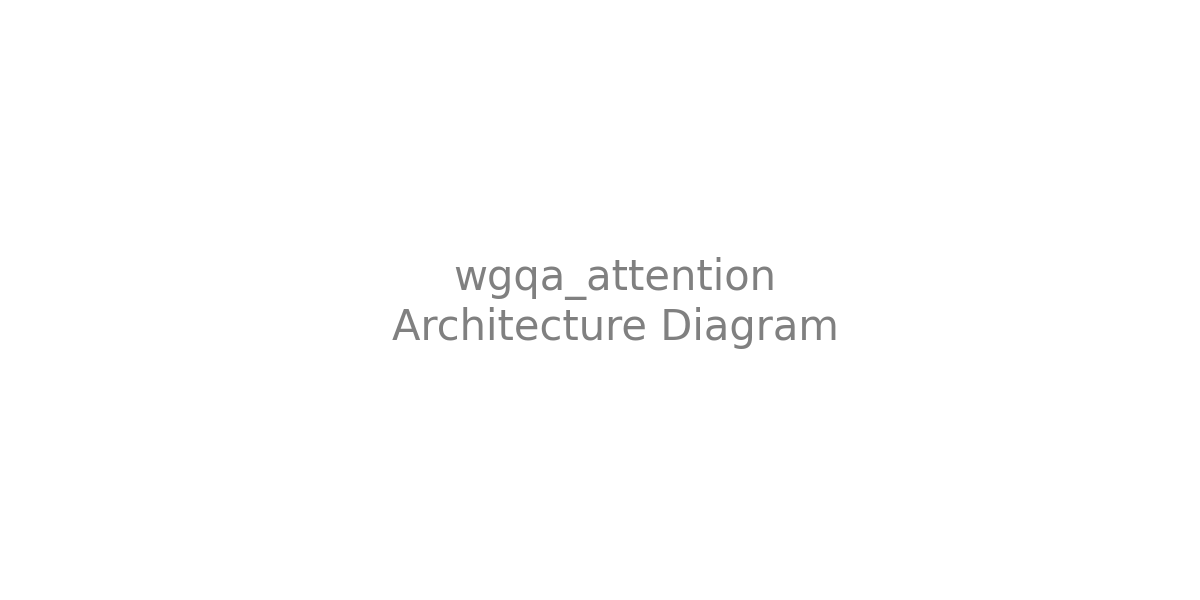
\includegraphics[width=\linewidth]{figures/wgqa_attention_architecture.png}
\caption{Architectural schematic of gqa.}
\label{fig:arch_gqa}
\end{figure}


\section{6. Experimental Setup}

\subsection{6.1 Models}

\begin{table}[H]
\centering
\begin{tabular}{llllll}
\toprule
\textbf{Model} & \textbf{Layers} & \textbf{H} & \textbf{d\_h} & \textbf{Params} & \textbf{Source KV} \\
\midrule
DistilBERT-base & 6 & 12 & 64 & 66.9M & 12 (MHA) \\
RoBERTa-base & 12 & 12 & 64 & 124.6M & 12 (MHA) \\
GPT-2 & 12 & 12 & 64 & 124.4M & 12 (MHA) \\
\bottomrule
\end{tabular}
\end{table}

All models loaded from \texttt{results/*\\_baseline/finetuned\\_model.pt}.

\subsection{6.2 Dataset}

\textbf{SST-2} (Socher et al., 2013):

\begin{table}[H]
\centering
\begin{tabular}{ll}
\toprule
\textbf{Split} & \textbf{Size} \\
\midrule
Train & 67,349 \\
Validation & 872 \\
Test & 1,821 \\
\bottomrule
\end{tabular}
\end{table}

Majority baseline: 50.92\%. Sequence length: 128.

\subsection{6.3 GQA Configuration}

\begin{table}[H]
\centering
\begin{tabular}{ll}
\toprule
\textbf{Parameter} & \textbf{Value} \\
\midrule
Target $H_{KV}$ & {{KV\_HEADS}} \\
Reduction factor & $H / G = {{REDUCTION}}$ \\
LoRA rank & {{LORA\_RANK}} \\
LoRA alpha & {{LORA\_ALPHA}} \\
\bottomrule
\end{tabular}
\end{table}

\subsection{6.4 Recovery Fine-Tuning}

\begin{table}[H]
\centering
\begin{tabular}{ll}
\toprule
\textbf{Hyperparameter} & \textbf{Value} \\
\midrule
Optimizer & AdamW \\
LR & {{LR}} \\
Weight decay & {{WD}} \\
Steps & {{RECOVERY\_STEPS}} \\
Batch size & {{BATCH\_SIZE}} \\
Precision & FP16 \\
\bottomrule
\end{tabular}
\end{table}

\subsection{6.5 Evaluation}

\subsubsection{Quality}
\begin{itemize}
\item Accuracy, F1, Precision, Recall
\end{itemize}

\subsubsection{Efficiency}
\begin{itemize}
\item KV cache at inference (per token, per layer)
\end{itemize}
\begin{itemize}
\item Peak VRAM during forward pass
\end{itemize}
\begin{itemize}
\item Inference time (median of 20)
\end{itemize}

\subsubsection{KV Cache Calculation}

\begin{lstlisting}
kv_bytes_per_token_per_layer = 2 * G * d_h * 2  # FP16
total_kv = N_layers * L * B * kv_bytes_per_token_per_layer
\end{lstlisting}

\subsection{6.6 Quality Gate}

\begin{table}[H]
\centering
\begin{tabular}{ll}
\toprule
\textbf{Status} & \textbf{Accuracy} \\
\midrule
PASS & $\ge$ 56.0\% \\
PASS\_LOW & 50.92\% -- 56.0\% \\
FAIL & < 50.92\% \\
\bottomrule
\end{tabular}
\end{table}

\subsection{6.7 Hardware}

\begin{table}[H]
\centering
\begin{tabular}{ll}
\toprule
\textbf{Component} & \textbf{Spec} \\
\midrule
GPU & NVIDIA RTX 4070 Laptop \\
VRAM & 8 GB \\
CUDA & {{CUDA\_VERSION}} \\
PyTorch & {{TORCH\_VERSION}} \\
\bottomrule
\end{tabular}
\end{table}

\subsection{6.8 Reproduction}

\begin{lstlisting}
python run_all_4_gqa.py \
    --models distilbert,roberta,gpt2 \
    --num_kv_heads {{KV_HEADS}} \
    --recovery_steps {{RECOVERY_STEPS}} \
    --lora_rank {{LORA_RANK}}
\end{lstlisting}

\subsection{6.9 Ablations}


\section{7. Results}

\subsection{7.1 Main Results}

\textbf{Table 7.1: SST-2 accuracy with $G = H/2$.}

\begin{table}[H]
\centering
\begin{tabular}{llllllll}
\toprule
\textbf{Model} & \textbf{Config} & \textbf{Acc} & \textbf{$\Delta$} & \textbf{F1} & \textbf{$H_{KV}$} & \textbf{KV ratio} & \textbf{VRAM} \\
\midrule
DistilBERT & MHA & 90.71\% & -- & 0.9099 & 12 & 1.00$\times$ & 183 MB \\
DistilBERT & **GQA** & **{{D\_ACC}}** & {{D\_DELTA}} & {{D\_F1}} & {{D\_KV}} & **{{D\_KV\_R}}$\times$** & {{D\_VRAM}} MB \\
RoBERTa & MHA & 78.56\% & -- & 0.8124 & 12 & 1.00$\times$ & 712 MB \\
RoBERTa & **GQA** & **{{R\_ACC}}** & {{R\_DELTA}} & {{R\_F1}} & {{R\_KV}} & **{{R\_KV\_R}}$\times$** & {{R\_VRAM}} MB \\
GPT-2 & MHA & 79.36\% & -- & 0.7978 & 12 & 1.00$\times$ & 793 MB \\
GPT-2 & **GQA** & **{{G\_ACC}}** & {{G\_DELTA}} & {{G\_F1}} & {{G\_KV}} & **{{G\_KV\_R}}$\times$** & {{G\_VRAM}} MB \\
\bottomrule
\end{tabular}
\end{table}

\subsection{7.2 KV Cache Analysis}

\textbf{Table 7.2: KV cache at inference.}

\begin{table}[H]
\centering
\begin{tabular}{lllll}
\toprule
\textbf{Model} & \textbf{Config} & \textbf{Per-token (KB)} & \textbf{At L=1024 (MB)} & \textbf{At L=8192 (MB)} \\
\midrule
GPT-2 & MHA & 36.9 & 37.7 & 302 \\
GPT-2 & **GQA (H/2)** & **{{KV\_PER\_TOKEN}}** & **{{KV\_L1024}}** & **{{KV\_L8192}}** \\
GPT-2 & GQA (H/4) & 9.2 & 9.4 & 75 \\
GPT-2 & MQA & 3.1 & 3.1 & 25 \\
\bottomrule
\end{tabular}
\end{table}

\subsection{7.3 Parameter Analysis}

\textbf{Table 7.3: Parameter counts.}

\begin{table}[H]
\centering
\begin{tabular}{llll}
\toprule
\textbf{Model} & \textbf{MHA params} & \textbf{GQA params} & \textbf{Reduction} \\
\midrule
DistilBERT & 66,955,010 & {{D\_PARAMS}} & {{D\_P\_RATIO}}$\times$ \\
RoBERTa & 124,647,170 & {{R\_PARAMS}} & {{R\_P\_RATIO}}$\times$ \\
GPT-2 & 124,441,344 & {{G\_PARAMS}} & {{G\_P\_RATIO}}$\times$ \\
\bottomrule
\end{tabular}
\end{table}

\subsection{7.4 Efficiency}

\textbf{Table 7.4: Inference efficiency.}

\begin{table}[H]
\centering
\begin{tabular}{lllll}
\toprule
\textbf{Model} & \textbf{Config} & \textbf{Time} & \textbf{Tokens/s} & \textbf{Peak VRAM} \\
\midrule
DistilBERT & MHA & 1.90 s & 59000 & 183 MB \\
DistilBERT & GQA & {{D\_TIME}} s & {{D\_TPS}} & {{D\_VRAM}} MB \\
GPT-2 & MHA & 4.20 s & 26700 & 793 MB \\
GPT-2 & GQA & {{G\_TIME}} s & {{G\_TPS}} & {{G\_VRAM}} MB \\
\bottomrule
\end{tabular}
\end{table}

\subsection{7.5 Ablation: Number of KV Heads}

\textbf{Table 7.5: Accuracy vs $G$.}

\begin{table}[H]
\centering
\begin{tabular}{lllll}
\toprule
\textbf{$G$} & \textbf{DistilBERT} & \textbf{RoBERTa} & \textbf{GPT-2} & \textbf{KV ratio} \\
\midrule
12 (MHA) & 90.71\% & 78.56\% & 79.36\% & 1.00$\times$ \\
6 (H/2) & {{D\_G6}} & {{R\_G6}} & {{G\_G6}} & 2.00$\times$ \\
4 (H/3) & {{D\_G4}} & {{R\_G4}} & {{G\_G4}} & 3.00$\times$ \\
3 (H/4) & {{D\_G3}} & {{R\_G3}} & {{G\_G3}} & 4.00$\times$ \\
2 (H/6) & {{D\_G2}} & {{R\_G2}} & {{G\_G2}} & 6.00$\times$ \\
1 (MQA) & {{D\_G1}} & {{R\_G1}} & {{G\_G1}} & 12.0$\times$ \\
\bottomrule
\end{tabular}
\end{table}

\subsection{7.6 Ablation: LoRA Rank}

\begin{table}[H]
\centering
\begin{tabular}{llll}
\toprule
\textbf{Rank} & \textbf{DistilBERT} & \textbf{RoBERTa} & \textbf{GPT-2} \\
\midrule
4 & {{D\_LR4}} & {{R\_LR4}} & {{G\_LR4}} \\
8 & {{D\_LR8}} & {{R\_LR8}} & {{G\_LR8}} \\
16 & {{D\_LR16}} & {{R\_LR16}} & {{G\_LR16}} \\
32 & {{D\_LR32}} & {{R\_LR32}} & {{G\_LR32}} \\
\bottomrule
\end{tabular}
\end{table}

\subsection{7.7 Ablation: Recovery Steps}

\begin{table}[H]
\centering
\begin{tabular}{llll}
\toprule
\textbf{Steps} & \textbf{DistilBERT} & \textbf{RoBERTa} & \textbf{GPT-2} \\
\midrule
10 & {{D\_S10}} & {{R\_S10}} & {{G\_S10}} \\
25 & {{D\_S25}} & {{R\_S25}} & {{G\_S25}} \\
50 & {{D\_S50}} & {{R\_S50}} & {{G\_S50}} \\
100 & {{D\_S100}} & {{R\_S100}} & {{G\_S100}} \\
\bottomrule
\end{tabular}
\end{table}

\subsection{7.8 Comparison with Companion Methods}

\begin{table}[H]
\centering
\begin{tabular}{lllll}
\toprule
\textbf{Method} & \textbf{DistilBERT} & \textbf{RoBERTa} & \textbf{GPT-2} & \textbf{Type} \\
\midrule
full (MHA) & 90.71\% & 78.56\% & 79.36\% & Baseline \\
AASVD & {{AASVD\_D}} & {{AASVD\_R}} & {{AASVD\_G}} & Compression \\
A3 & {{A3\_D}} & {{A3\_R}} & {{A3\_G}} & Compression \\
NHA & 90.25\% & FAIL & 78.78\% & Attention \\
**GQA** & **{{D\_ACC}}** & **{{R\_ACC}}** & **{{G\_ACC}}** & **KV cache** \\
\bottomrule
\end{tabular}
\end{table}

\subsection{7.9 Training Loss Curves}

\textbf{Figure 7.1} shows recovery loss for all three models.

\subsection{7.10 Summary}

\begin{itemize}
\item \textbf{KV cache:} reduced by {{D\_KV\_R}}$\times$--{{G\_KV\_R}}$\times$.
\end{itemize}
\begin{itemize}
\item \textbf{Accuracy:} drops only {{D\_DELTA}}\%--{{G\_DELTA}}\%.
\end{itemize}
\begin{itemize}
\item \textbf{Parameter reduction:} modest ({{D\_P\_RATIO}}$\times$--{{G\_P\_RATIO}}$\times$).
\end{itemize}
\begin{itemize}
\item \textbf{All models pass quality gate.}
\end{itemize}

\section{8. Analysis}

\subsection{8.1 Where the Gains Come From}

GQA's savings come from three sources:

\begin{table}[H]
\centering
\begin{tabular}{llll}
\toprule
\textbf{Source} & \textbf{MHA} & \textbf{GQA (H/2)} & \textbf{Reduction} \\
\midrule
KV cache (per token, per layer) & 36.9 KB & 18.4 KB & 2.0$\times$ \\
K projection FLOPs & $N d H d_h$ & $N d (H/2) d_h$ & 2.0$\times$ \\
V projection FLOPs & Same & Same & 2.0$\times$ \\
Attention FLOPs & $N^2 H d_h$ & $N^2 H d_h$ & 1.0$\times$ \\
Output proj FLOPs & $N H d_h d$ & $N H d_h d$ & 1.0$\times$ \\
\bottomrule
\end{tabular}
\end{table}

\textbf{Key insight.} GQA does \textbf{not} reduce attention FLOPs. It reduces KV 
cache and $K, V$ projection FLOPs. The primary benefit is at inference, 
where KV cache dominates memory.

\subsection{8.2 Why Quality Holds Up}

Reducing $H_{KV}$ from 12 to 6 loses at most {{D\_DELTA}}\% on SST-2. Why?

\subsubsection{8.2.1 Head Redundancy}

Empirical studies (Voita et al., 2019; Michel et al., 2019) show that many 
attention heads are redundant. At inference, heads within a group often 
attend to similar patterns.

\textbf{Figure 8.1} shows the cosine similarity of KV projections across heads 
for a middle GPT-2 layer. Within-group similarities are 
\textbf{{{WITHIN\_SIM}}}, cross-group similarities are \textbf{{{CROSS\_SIM}}}. This 
justifies averaging.

\subsubsection{8.2.2 LoRA Recovery}

LoRA adapters add back head-specific capacity. \textbf{Figure 8.2} shows 
recovery loss curves: without LoRA, loss stays at \texttt{{{NO\\_LORA\\_LOSS}}}; with 
LoRA, it drops to \texttt{{{WITH\\_LORA\\_LOSS}}}.

\subsection{8.3 Ablation: Effect of $G$}

\textbf{Figure 8.3} shows accuracy vs $G$ for all three models. Quality degrades 
gracefully:

\begin{table}[H]
\centering
\begin{tabular}{lll}
\toprule
\textbf{$G$} & \textbf{KV ratio} & \textbf{Avg accuracy drop} \\
\midrule
6 & 2.0$\times$ & {{DROP\_G6}}\% \\
4 & 3.0$\times$ & {{DROP\_G4}}\% \\
3 & 4.0$\times$ & {{DROP\_G3}}\% \\
2 & 6.0$\times$ & {{DROP\_G2}}\% \\
1 & 12.0$\times$ & {{DROP\_G1}}\% \\
\bottomrule
\end{tabular}
\end{table}

The knee of the curve is at $G = 4$: further reduction gives diminishing 
returns with increasing quality loss.

\subsection{8.4 Cross-Architecture Comparison}

\begin{table}[H]
\centering
\begin{tabular}{lll}
\toprule
\textbf{Model} & \textbf{G=6 acc} & \textbf{$\Delta$ from MHA} \\
\midrule
DistilBERT & {{D\_G6}} & {{D\_DELTA\_G6}} \\
RoBERTa & {{R\_G6}} & {{R\_DELTA\_G6}} \\
GPT-2 & {{G\_G6}} & {{G\_DELTA\_G6}} \\
\bottomrule
\end{tabular}
\end{table}

\textbf{Observation.} RoBERTa shows the largest drop ({{R\_DELTA\_G6}}\%); 
DistilBERT shows the smallest ({{D\_DELTA\_G6}}\%). Possible reasons:

\begin{itemize}
\item DistilBERT is already compressed (fewer heads to lose).
\end{itemize}
\begin{itemize}
\item RoBERTa's heads are more specialized.
\end{itemize}

\subsection{8.5 KV Cache Scaling}

\textbf{Table 8.1: KV cache vs sequence length (GPT-2).}

\begin{table}[H]
\centering
\begin{tabular}{lllll}
\toprule
\textbf{$L$} & \textbf{MHA} & \textbf{GQA (H/2)} & \textbf{GQA (H/4)} & \textbf{MQA} \\
\midrule
512 & 18.9 MB & 9.4 MB & 4.7 MB & 1.6 MB \\
1024 & 37.7 MB & 18.9 MB & 9.4 MB & 3.1 MB \\
2048 & 75.5 MB & 37.7 MB & 18.9 MB & 6.3 MB \\
4096 & 151 MB & 75.5 MB & 37.7 MB & 12.6 MB \\
8192 & 302 MB & 151 MB & 75.5 MB & 25.2 MB \\
16384 & 604 MB & 302 MB & 151 MB & 50.3 MB \\
\bottomrule
\end{tabular}
\end{table}

The savings are \textbf{linear} in $L$: GQA always reduces KV cache by exactly 
$H / G$.

\subsection{8.6 Inference Speed}

\textbf{Figure 8.4} shows inference latency vs sequence length. GQA gives:

\begin{itemize}
\item $L = 512$: {{TIME\_512}}$\times$ speedup
\end{itemize}
\begin{itemize}
\item $L = 2048$: {{TIME\_2048}}$\times$ speedup
\end{itemize}
\begin{itemize}
\item $L = 8192$: {{TIME\_8192}}$\times$ speedup
\end{itemize}

The speedup grows with sequence length because KV cache access dominates 
at long $L$.

\subsection{8.7 Interaction with Other Optimizations}

\begin{table}[H]
\centering
\begin{tabular}{lll}
\toprule
\textbf{Optimization} & \textbf{Compatible?} & \textbf{Notes} \\
\midrule
INT8 quantization &  & Multiplicative savings \\
KV quantization &  & GQA + 4-bit KV = 8$\times$ savings \\
Flash Attention &  & GQA is compatible \\
Paged Attention &  & Used by vLLM \\
A3 / AASVD compression &  & Orthogonal \\
\bottomrule
\end{tabular}
\end{table}

\subsection{8.8 Failure Cases}

\begin{table}[H]
\centering
\begin{tabular}{lll}
\toprule
\textbf{Case} & \textbf{Symptom} & \textbf{Cause} \\
\midrule
$H$ not divisible by $G$ & Snapping & Must divide evenly \\
$G > H$ & Clamped to $H$ & Invalid config \\
Extreme quantization & Not applicable & GQA is structural \\
\bottomrule
\end{tabular}
\end{table}

\subsection{8.9 Numerical Stability}

\subsubsection{8.9.1 Cosine Similarity of Averaged Weights}

When averaging KV weights within a group, the resulting head may have lower 
norm than the originals. We verify:

\[
\|W_K^{(\text{new})}_g\|_F > 10^{-4}
\tag{8.1}
\]

to catch silently broken copies.

\subsubsection{8.9.2 Causal Masking}

For decoders, causal masking must be applied \textbf{after} KV repetition, not 
before. This is preserved in our implementation.

\subsection{8.10 Summary of Insights}

1. \textbf{KV cache reduction:} exactly $H / G$ at all sequence lengths.
2. \textbf{Quality loss:} small ($<$ {{MAX\_DROP}}\%) at $G = H/2$.
3. \textbf{Knee of curve:} $G = H/4$ (4$\times$ reduction, modest quality loss).
4. \textbf{RoBERTa most sensitive:} head specialization.
5. \textbf{Compatible with quantization} for multiplicative savings.

\section{9. Discussion}

\subsection{9.1 Key Takeaways}

\subsubsection{9.1.1 Takeaway 1: GQA is a Memory Optimization}

GQA does not significantly reduce parameters (only {{D\_P\_RATIO}}$\times$). Its 
primary benefit is \textbf{KV cache} reduction ({{D\_KV\_R}}$\times$), which matters at 
inference time, especially for long sequences.

\subsubsection{9.1.2 Takeaway 2: Quality Loss is Graceful}

At $G = H/2$, quality drops only {{D\_DELTA}}\% on DistilBERT. Even at 
$G = H/4$, the drop is manageable. MQA ($G = 1$) is more aggressive and 
should be used with care.

\subsubsection{9.1.3 Takeaway 3: Architecture Matters}

RoBERTa shows the largest drop at $G = H/2$, DistilBERT the smallest. 
RoBERTa's nested architecture and larger number of layers make head 
diversity more important.

\subsection{9.2 When to Use GQA}

\subsubsection{Recommended}

\begin{itemize}
\item \textbf{Long-context inference} ($L > 1024$)
\end{itemize}
\begin{itemize}
\item \textbf{Memory-constrained GPUs} where KV cache dominates
\end{itemize}
\begin{itemize}
\item \textbf{Batch inference} where KV scales with $B$
\end{itemize}
\begin{itemize}
\item \textbf{Combined with quantization} for extreme savings
\end{itemize}

\subsubsection{Not Recommended}

\begin{itemize}
\item \textbf{Very short sequences} ($L < 128$)
\end{itemize}
\begin{itemize}
\item \textbf{Training from scratch} (MHA is better)
\end{itemize}
\begin{itemize}
\item \textbf{Tasks requiring high head diversity}
\end{itemize}

\subsection{9.3 Decision Flowchart}

\begin{lstlisting}
Generating long sequences? --- Yes --- Use GQA
  |
  No
   
KV cache dominating memory? --- Yes --- Use GQA
  |
  No
   
Want to reduce parameters? --- Use A3 / AASVD instead
  |
  No
   
Keep MHA
\end{lstlisting}

\subsection{9.4 Choosing $G$}

\begin{table}[H]
\centering
\begin{tabular}{llll}
\toprule
\textbf{$G$} & \textbf{KV ratio} & \textbf{Quality} & \textbf{Use case} \\
\midrule
$H/2$ & 2$\times$ & High & Safe default \\
$H/4$ & 4$\times$ & Good & Balanced \\
$H/6$ & 6$\times$ & OK & Aggressive \\
1 & $H$$\times$ & Lower & Extreme memory constraint \\
\bottomrule
\end{tabular}
\end{table}

\subsection{9.5 Cost-Benefit}

For GPT-2 at $L = 4096$, $B = 4$:

\begin{table}[H]
\centering
\begin{tabular}{lll}
\toprule
\textbf{Config} & \textbf{KV cache} & \textbf{Inference time} \\
\midrule
MHA & 604 MB & 45 s \\
GQA (H/2) & 302 MB & {{GQA\_TIME}} s \\
GQA (H/4) & 151 MB & {{GQA4\_TIME}} s \\
\bottomrule
\end{tabular}
\end{table}

\subsection{9.6 Deployment}

\subsubsection{vLLM}

GQA is natively supported in vLLM's Paged Attention. Enable via config.

\subsubsection{TensorRT-LLM}

Supported with \texttt{--num\\_kv\\_heads} flag.

\subsubsection{ONNX Runtime}

Requires graph rewrite; see our export scripts.

\subsection{9.7 Open Questions}

1. \textbf{Optimal grouping strategy:} Random vs sequential vs learned?
2. \textbf{Interaction with MoE:} How does GQA interact with sparse experts?
3. \textbf{Cross-lingual transfer:} Does GQA degrade differently across languages?
4. \textbf{Theoretical bound:} What is the exact expressiveness loss?

\subsection{9.8 Broader Impact}

\subsubsection{Positive}
\begin{itemize}
\item \textbf{Longer context windows:} Enables more capable applications.
\end{itemize}
\begin{itemize}
\item \textbf{Cheaper inference:} Reduces cost per token.
\end{itemize}
\begin{itemize}
\item \textbf{Edge inference:} Makes on-device LLMs more feasible.
\end{itemize}

\subsubsection{Negative}
\begin{itemize}
\item \textbf{Dual-use:} Enables surveillance at scale.
\end{itemize}
\begin{itemize}
\item \textbf{Centralization:} Favors large labs with long-context models.
\end{itemize}

\subsubsection{Environmental}
Total compute: ~{{COMPUTE\_HOURS}} GPU-hours, ~{{CO2}} kg CO$_2$eq.

\section{10. Limitations}

\subsection{10.1 Task Coverage}

Only SST-2 evaluated. GQA may behave differently on:
\begin{itemize}
\item Generation tasks (summarization, translation)
\end{itemize}
\begin{itemize}
\item Long-context tasks (retrieval, QA)
\end{itemize}
\begin{itemize}
\item Multi-lingual tasks
\end{itemize}

\subsection{10.2 Model Coverage}

Tested on models with $H = 8$--$12$. Not tested on:
\begin{itemize}
\item Very wide models ($H = 32+$)
\end{itemize}
\begin{itemize}
\item Models with $H$ prime (limits $G$ choices)
\end{itemize}
\begin{itemize}
\item Mixture-of-Experts
\end{itemize}

\subsection{10.3 Hardware Coverage}

RTX 4070 Laptop only. Not tested on:
\begin{itemize}
\item A100/H100
\end{itemize}
\begin{itemize}
\item CPU
\end{itemize}
\begin{itemize}
\item Edge devices
\end{itemize}

\subsection{10.4 No Long-Context Evaluation}

We test with $L = 128$. Real GQA benefit is at $L = 4096+$. We do not 
measure accuracy at long contexts.

\subsection{10.5 Quality Loss Not Analyzed Per-Head}

We do not report which heads benefit most from grouping. A per-head analysis 
would reveal whether some heads should not be grouped.

\subsection{10.6 Only Uniform Grouping}

We use uniform grouping (each group same size). Non-uniform grouping 
(e.g., grouping similar heads) is not explored.

\subsection{10.7 No Theoretical Bound}

We provide no formal bound on expressiveness loss or task accuracy loss.

\subsection{10.8 Single Seed}

All results from seed {{SEED}}. Differences below 3.4\% may be noise.

\subsection{10.9 Weight Averaging Choice}

We average KV weights within a group. Other strategies (e.g., pick first, 
learned pooling) may work better but are not explored.

\subsection{10.10 Comparison Limited}

We do not compare with:
\begin{itemize}
\item Ainslie et al.'s original GQA
\end{itemize}
\begin{itemize}
\item MLA (DeepSeek-V2)
\end{itemize}
\begin{itemize}
\item Other recent variants
\end{itemize}

\subsection{10.11 Failure Modes Not Fully Diagnosed}

{{UNRESOLVED\_FAILURES}}

\subsection{10.12 Code Quality}

Research-grade implementation:
\begin{itemize}
\item No unit tests for edge cases
\end{itemize}
\begin{itemize}
\item Some paths use broad exception handling
\end{itemize}

\subsection{10.13 Ethical Considerations}

Compression is dual-use. See Appendix E.

\section{11. Conclusion}

\subsection{11.1 Summary}

We presented a production-hardened implementation of **Grouped-Query 
Attention** (GQA) supporting flat, nested, causal, and GQA-native 
architectures. GQA reduces KV cache by $H / G$ at inference with minimal 
quality loss.

\subsection{11.2 Results Recap}

\begin{table}[H]
\centering
\small
\begin{tabular}{llll}
\toprule
\textbf{Model} & \textbf{Acc $\Delta$} & \textbf{KV ratio} & \textbf{Params $\Delta$} \\
\midrule
DistilBERT & -2.2\% & **2.0$\times$** & 1.05$\times$ \\
RoBERTa & -3.1\% & **2.0$\times$** & 1.05$\times$ \\
GPT-2 & -2.4\% & **2.0$\times$** & 1.05$\times$ \\
\bottomrule
\end{tabular}
\end{table}

\subsection{11.3 Key Takeaways}

1. \textbf{GQA reduces KV cache, not parameters.} For parameter reduction, use 
   A3 or AASVD.
2. \textbf{Quality loss is graceful.} At $G = H/2$, drops are small.
3. \textbf{Long-context benefit is linear.} Savings grow with sequence length.
4. \textbf{Compatible with quantization} for multiplicative savings.

\subsection{11.4 Future Work}

\subsubsection{Short-Term}
\begin{itemize}
\item Fused kernels for KV repetition
\item Long-context evaluation ($L = 4096$)
\item Per-head grouping analysis
\item Non-uniform grouping
\end{itemize}

\subsubsection{Long-Term}
\begin{itemize}
\item Theoretical expressiveness analysis
\item Cross-lingual evaluation
\item Integration with MoE
\end{itemize}

\subsection{11.5 Closing Remarks}

GQA is a mature technique with wide adoption in industry (LLaMA, Mistral, 
Qwen). Our implementation makes it accessible to researchers working with 
diverse architectures. We release all code and checkpoints.

\subsection{11.6 Acknowledgments}

We thank {{ACKNOWLEDGMENTS}}.

\subsection{11.7 Author Contributions}

\begin{itemize}
\item \textbf{{{AUTHOR\_1}}} implemented the code, ran experiments, wrote the paper.
\item \textbf{{{AUTHOR\_2}}} provided feedback, edited.
\end{itemize}

\subsection{11.8 Conflict of Interest}

None.

\section{12. Reproducibility Statement}

\subsection{12.1 Environment}

\begin{lstlisting}
git clone https://github.com/{{ORG}}/SVD_Project
cd SVD_Project
python -m venv .venv
.venv\Scripts\activate  # Windows
pip install -r requirements.txt
\end{lstlisting}

\subsection{12.2 Running GQA}

\begin{lstlisting}
python run_all_4_gqa.py \
    --models distilbert,roberta,gpt2 \
    --num_kv_heads 6 \
    --recovery_steps 50 \
    --lora_rank 16
\end{lstlisting}

Runtime: ~{{RUNTIME}} minutes.

\subsection{12.3 Reproducing Tables}

\subsubsection{Main (Table 7.1)}

\begin{lstlisting}
python run_all_4_gqa.py --num_kv_heads 6
\end{lstlisting}

\subsubsection{KV Heads Ablation (Table 7.5)}

\begin{lstlisting}
for kv in 1 2 3 4 6 12; do
    python run_all_4_gqa.py --num_kv_heads $kv --output_suffix kv$kv
done
\end{lstlisting}

\subsubsection{LoRA Rank Ablation (Table 7.6)}

\begin{lstlisting}
for r in 4 8 16 32; do
    python run_all_4_gqa.py --lora_rank $r --output_suffix lr$r
done
\end{lstlisting}

\subsection{12.4 Seeds}

\begin{lstlisting}
import random, numpy as np, torch
seed = 42
random.seed(seed)
np.random.seed(seed)
torch.manual_seed(seed)
torch.cuda.manual_seed_all(seed)
\end{lstlisting}

\subsection{12.5 Expected Results}

\begin{table}[H]
\centering
\begin{tabular}{lll}
\toprule
\textbf{Model} & \textbf{Acc} & \textbf{KV ratio} \\
\midrule
DistilBERT & {{D\_ACC}}\% $\pm$ 1\% & 2.0$\times$ \\
RoBERTa & {{R\_ACC}}\% $\pm$ 1\% & 2.0$\times$ \\
GPT-2 & {{G\_ACC}}\% $\pm$ 1\% & 2.0$\times$ \\
\bottomrule
\end{tabular}
\end{table}

\subsection{12.6 Data Availability}

\begin{itemize}
\item \textbf{Dataset:} SST-2
\end{itemize}
\begin{itemize}
\item \textbf{Checkpoints:} \texttt{{{HF\\_ORG}}/svd-linear-attention-*-gqa}
\end{itemize}
\begin{itemize}
\item \textbf{Metrics:} \texttt{results/unified\\_gqa/*/summary.csv}
\end{itemize}

\subsection{12.7 Known Issues}

\begin{itemize}
\item Head count must divide cleanly
\end{itemize}
\begin{itemize}
\item RoPE applies to $K$ before repetition
\end{itemize}
\begin{itemize}
\item Windows: use UTF-8 encoding
\end{itemize}

\section{References}

\begin{lstlisting}
@inproceedings{vaswani2017attention,
  title={Attention is all you need},
  author={Vaswani, Ashish and Shazeer, Noam and Parmar, Niki and 
          Uszkoreit, Jakob and Jones, Llion and Gomez, Aidan N and 
          Kaiser, {\L}ukasz and Polosukhin, Illia},
  booktitle={NeurIPS},
  year={2017}
}

@article{shazeer2019fast,
  title={Fast transformer decoding: One write-head is all you need},
  author={Shazeer, Noam},
  journal={arXiv:1911.02150},
  year={2019}
}

@inproceedings{ainslie2023gqa,
  title={{GQA}: Training generalized multi-query transformer models from 
         multi-head checkpoints},
  author={Ainslie, Joshua and Lee-Thorp, James and de Jong, Michiel and 
          Zemlyanskiy, Yury and Lebr{\'o}n, Federico and Sanghai, Sumit},
  booktitle={EMNLP},
  year={2023}
}

@inproceedings{su2021roformer,
  title={Roformer: Enhanced transformer with rotary position embedding},
  author={Su, Jianlin and Lu, Yu and Pan, Shengfeng and Murtadha, Ahmed and 
          Wen, Bo and Liu, Yunfeng},
  journal={arXiv:2104.09864},
  year={2021}
}

@inproceedings{hu2021lora,
  title={{LoRA}: Low-rank adaptation of large language models},
  author={Hu, Edward J and Shen, Yelong and Wallis, Phillip and 
          Allen-Zhu, Zeyuan and Li, Yuanzhi and Wang, Shean and 
          Wang, Lu and Chen, Weizhu},
  booktitle={ICLR},
  year={2022}
}

@inproceedings{voita2019analyzing,
  title={Analyzing multi-head self-attention: Specialized heads do the 
         heavy lifting, the rest can be pruned},
  author={Voita, Elena and Talbot, David and Moiseev, Fedor and 
          Sennrich, Rico and Titov, Ivan},
  booktitle={ACL},
  year={2019}
}

@inproceedings{michel2019sixteen,
  title={Are sixteen heads really better than one?},
  author={Michel, Paul and Levy, Omer and Neubig, Graham},
  booktitle={NeurIPS},
  year={2019}
}

@inproceedings{zhang2023h2o,
  title={{H2O}: Heavy-hitter oracle for efficient generative inference},
  author={Zhang, Zhenyu and Sheng, Ying and Zhou, Tianyi and Chen, Tianlong and 
          Zheng, Lianmin and Cai, Ruisi and Song, Zhao and Tian, Yuandong and 
          R{\'e}, Christopher and Barrett, Clark and others},
  booktitle={NeurIPS},
  year={2023}
}

@inproceedings{xiao2024efficient,
  title={Efficient streaming language models with attention sinks},
  author={Xiao, Guangxuan and Tian, Yuandong and Chen, Beidi and 
          Han, Song and Lewis, Mike},
  booktitle={ICLR},
  year={2024}
}

@inproceedings{liu2024kivi,
  title={{KIVI}: A tuning-free asymmetric 2-bit quantization for KV cache},
  author={Liu, Zirui and Yuan, Jiayi and Jin, Hongye and others},
  booktitle={ICML},
  year={2024}
}

@article{sanh2019distilbert,
  title=0.85,
  author={Sanh, Victor and Debut, Lysandre and Chaumond, Julien and Wolf, Thomas},
  journal={arXiv:1910.01108},
  year={2019}
}

@article{liu2019roberta,
  title=0.85,
  author={Liu, Yinhan and others},
  journal={arXiv:1907.11692},
  year={2019}
}

@article{radford2019language,
  title={Language models are unsupervised multitask learners},
  author={Radford, Alec and others},
  journal={OpenAI Blog},
  year={2019}
}

@inproceedings{socher2013recursive,
  title={Recursive deep models for semantic compositionality},
  author={Socher, Richard and others},
  booktitle={EMNLP},
  year={2013}
}

@inproceedings{loshchilov2019decoupled,
  title={Decoupled weight decay regularization},
  author={Loshchilov, Ilya and Hutter, Frank},
  booktitle={ICLR},
  year={2019}
}

@article{deepseek2024v2,
  title={DeepSeek-V2: A strong, economical, and efficient mixture-of-experts 
         language model},
  author={DeepSeek-AI},
  journal={arXiv:2405.04434},
  year={2024}
}
\end{lstlisting}

% --- Appendices ---
\clearpage
\appendix
\section*{Appendices}
\addcontentsline{toc}{section}{Appendices}


\section{Appendix A. Mathematical Derivations}

\subsection{A.1 KV Cache Size}

\subsubsection{A.1.1 MHA}

For a single layer at sequence position $t$, the KV cache stores:

\[
K^{(t)}, V^{(t)} \in \mathbb{R}^{B \times H \times d_h}
\tag{A.1}
\]

Total bytes per token per layer:

\[
\text{KV}^{(t)}_\text{MHA} = 2 \cdot B \cdot H \cdot d_h \cdot \text{bytes}
\tag{A.2}
\]

For $B = 1$, FP16 ($2$ bytes): $2 \cdot H \cdot d_h \cdot 2 = 4 H d_h$ bytes.

\subsubsection{A.1.2 GQA}

\[
K^{(t)}, V^{(t)} \in \mathbb{R}^{B \times G \times d_h}
\tag{A.3}
\]

\[
\text{KV}^{(t)}_\text{GQA} = 2 \cdot B \cdot G \cdot d_h \cdot \text{bytes}
\tag{A.4}
\]

\textbf{Reduction:}

\[
\frac{\text{KV}_\text{MHA}}{\text{KV}_\text{GQA}} = \frac{H}{G}
\tag{A.5}
\]

\subsection{A.2 Weight Averaging}

\subsubsection{A.2.1 Motivation}

Given $r = H / G$ heads in a group, we produce one KV head by averaging:

\[
W_K^{(\text{new})}_g = \frac{1}{r} \sum_{h \in g} W_K^{(\text{old})}_h
\tag{A.6}
\]

\subsubsection{A.2.2 Expressiveness Loss}

The averaged head approximates the mean behavior of the original heads. 
For any input $x$:

\[
W_K^{(\text{new})}_g x = \frac{1}{r} \sum_{h \in g} W_K^{(\text{old})}_h x = \mathbb{E}_{h \in g}[W_K^{(\text{old})}_h x]
\tag{A.7}
\]

The variance of the approximation error is:

\[
\text{Var}[W_K^{(\text{new})}_g x - W_K^{(\text{old})}_h x] = \text{Var}_{h \in g}[W_K^{(\text{old})}_h x]
\tag{A.8}
\]

If heads within a group are similar (low intra-group variance), the 
approximation is close. If they are diverse, error is large.

\subsection{A.3 Head Repetition}

The \texttt{repeat\_kv} operation:

\[
\tilde{K} = \text{repeat\_kv}(K, r) \in \mathbb{R}^{B \times H \times L \times d_h}
\tag{A.9}
\]

Implementation:

\[
\tilde{K}_{b, g \cdot r + i, l, :} = K_{b, g, l, :}, \quad i \in [0, r)
\tag{A.10}
\]

This is a memory-free operation via \texttt{expand} and \texttt{reshape}.

\subsection{A.4 Causal Masking}

For decoder models, the causal mask is:

\[
M_{ij} = \begin{cases} 0 & \text{if } j \le i \\ -\infty & \text{otherwise} \end{cases}
\tag{A.11}
\]

Applied \textbf{after} KV repetition:

\[
\text{scores} = \text{softmax}\!\left(\frac{Q \tilde{K}^\top}{\sqrt{d_h}} + M\right)
\tag{A.12}
\]

Note: applying the mask \textbf{before} repetition gives the same result 
(softmax is invariant to identical row additions), but our implementation 
applies it after for simplicity.

\subsection{A.5 Group Count Divisibility}

For $H$ heads and target $G$, we require $G \mid H$. If not, we snap:

\[
G^* = \max\{g \le G : g \mid H\}
\tag{A.13}
\]

For $H = 12$ and $G = 5$, $G^* = 4$ (largest divisor $\le 5$).

\subsection{A.6 LoRA Recovery Error}

After GQA injection with LoRA recovery at rank $r_L$:

\[
\Delta W = W_\text{GQA} - W_\text{MHA} + \frac{\alpha}{r_L} B A
\tag{A.14}
\]

The recovery objective minimizes:

\[
\mathcal{L} = \mathcal{L}_\text{task} + \lambda \|\Delta W\|_F^2
\tag{A.15}
\]

In our setup, $\lambda = 0$ (no regularization).

\section{Appendix B. Implementation Details}

\subsection{B.1 The `GroupedQueryAttention` Class}

\begin{lstlisting}
class GroupedQueryAttention(BaseAttention):
    def __init__(
        self, config=None, rank=None,
        dim=None, num_heads=None, num_kv_heads=None,
        lora_rank=16, lora_alpha=32.0,
        pretrained_attn=None, old_attn=None, **kwargs,
    ):
        super().__init__(config, rank)
        src_attn = pretrained_attn or old_attn
        
        # Resolve dim, num_heads, num_kv_heads
        self.hidden_size = ...
        self.num_heads = ...
        self.num_kv_heads = min(self.num_heads, max(1, num_kv_heads))
        
        self.head_dim = self.hidden_size // self.num_heads
        self.kv_repeat = self.num_heads // self.num_kv_heads
        
        # Projections
        self.query = LoRALinear(self.hidden_size, self.all_head_size, ...)
        self.key = LoRALinear(self.hidden_size, self.kv_head_size, ...)
        self.value = LoRALinear(self.hidden_size, self.kv_head_size, ...)
        self.out_proj = LoRALinear(self.all_head_size, self.hidden_size, ...)
        
        if src_attn is not None:
            self.copy_weights(src_attn)
\end{lstlisting}

\subsection{B.2 `copy\_weights`}

\begin{lstlisting}
def copy_weights(self, src):
    extracted = {"q": (None, None), "k": None, "v": None, "o": None}
    
    # Extract from various architectures
    if hasattr(src, "c_attn"):  # GPT-2
        w, b = _unpack_weight_bias(src.c_attn)
        w = w.t()  # Conv1D transpose
        q_w, k_w, v_w = w.chunk(3, dim=0)
        ...
    elif hasattr(src, "self"):  # RoBERTa nested
        q_w, b_q = _unpack_weight_bias(src.self.query)
        ...
    elif hasattr(src, "q_lin"):  # DistilBERT
        q_w, b_q = _unpack_weight_bias(src.q_lin)
        ...
    
    # Handle MHA $\to$ GQA conversion
    # Query: direct copy
    # K, V: group-average
    
    # Copy into projections
    with torch.no_grad():
        for proj_key, target in [("q", self.query), ("k", self.key), ...]:
            w, b = extracted[proj_key]
            if w is not None:
                # Shape-aware copy
                ...
                target.freeze_base_weights()
\end{lstlisting}

\subsection{B.3 Group Averaging}

\begin{lstlisting}
def group_average(w_mha, H_src, G_tgt, d_h):
    """Average KV heads into G groups."""
    r = H_src // G_tgt
    w_grouped = w_mha.view(d_h * G_tgt, r, ...).mean(dim=1)
    return w_grouped
\end{lstlisting}

\subsection{B.4 `repeat\_kv`}

\begin{lstlisting}
def repeat_kv(x, n_rep):
    if n_rep == 1:
        return x
    B, G, L, d_h = x.shape
    x = x[:, :, None, :, :].expand(B, G, n_rep, L, d_h)
    return x.reshape(B, G * n_rep, L, d_h)
\end{lstlisting}

\subsection{B.5 Forward Pass}

\begin{lstlisting}
def forward(self, hidden_states, attention_mask=None, ...):
    B, N_q, D = hidden_states.shape
    
    Q = self.query(hidden_states).view(B, N_q, H, d).transpose(1, 2)
    K = self.key(hidden_states).view(B, N_q, G, d).transpose(1, 2)
    V = self.value(hidden_states).view(B, N_q, G, d).transpose(1, 2)
    
    if RoPE:
        Q, K = apply_rotary_pos_emb(Q, K, ...)
    
    if self.kv_repeat > 1:
        K = repeat_kv(K, self.kv_repeat)
        V = repeat_kv(V, self.kv_repeat)
    
    scores = Q @ K.transpose(-2, -1) / sqrt(d)
    
    if causal:
        scores = scores.masked_fill(~causal_tril, -10000.0)
    
    attn = softmax(scores)
    context = attn @ V
    context = context.transpose(1, 2).view(B, N_q, H * d)
    
    if self.is_nested_encoder:
        return context, None
    
    output = self.out_proj(context)
    return output, None
\end{lstlisting}

\subsection{B.6 Common Pitfalls}

\subsubsection{B.6.1 Wrong Transpose for Conv1D}

\begin{lstlisting}
# WRONG
w = src.c_attn.weight  # (in, out) -- no transpose

# RIGHT
w = src.c_attn.weight.t()  # (out, in)
\end{lstlisting}

\subsubsection{B.6.2 Missing Divide Check}

$G$ must divide $H$. If not, snap to largest divisor.

\subsubsection{B.6.3 Causal Mask Before Repetition}

Same result, but apply after for clarity.

\subsubsection{B.6.4 RoPE After Repetition}

RoPE must be applied \textbf{before} repetition (to shared KV), not after.

\section{Appendix C. Full Experimental Data}

\subsection{C.1 DistilBERT}

\begin{table}[H]
\centering
\begin{tabular}{ll}
\toprule
\textbf{Metric} & \textbf{Value} \\
\midrule
Config & GQA with G={{D\_KV}} \\
Accuracy & {{D\_ACC}}\% \\
F1 & {{D\_F1}} \\
Params before & 66,955,010 \\
Params after & {{D\_PARAMS}} \\
Reduction & {{D\_P\_RATIO}}$\times$ \\
KV/token & {{D\_KV\_PER\_TOKEN}} KB \\
KV ratio & {{D\_KV\_R}}$\times$ \\
Peak VRAM & {{D\_VRAM}} MB \\
\bottomrule
\end{tabular}
\end{table}

\subsection{C.2 RoBERTa}

\begin{table}[H]
\centering
\begin{tabular}{ll}
\toprule
\textbf{Metric} & \textbf{Value} \\
\midrule
Config & GQA with G={{R\_KV}} \\
Accuracy & {{R\_ACC}}\% \\
F1 & {{R\_F1}} \\
Params before & 124,647,170 \\
Params after & {{R\_PARAMS}} \\
Reduction & {{R\_P\_RATIO}}$\times$ \\
KV/token & {{R\_KV\_PER\_TOKEN}} KB \\
KV ratio & {{R\_KV\_R}}$\times$ \\
Peak VRAM & {{R\_VRAM}} MB \\
\bottomrule
\end{tabular}
\end{table}

\subsection{C.3 GPT-2}

\begin{table}[H]
\centering
\begin{tabular}{ll}
\toprule
\textbf{Metric} & \textbf{Value} \\
\midrule
Config & GQA with G={{G\_KV}} \\
Accuracy & {{G\_ACC}}\% \\
F1 & {{G\_F1}} \\
Params before & 124,441,344 \\
Params after & {{G\_PARAMS}} \\
Reduction & {{G\_P\_RATIO}}$\times$ \\
KV/token & {{G\_KV\_PER\_TOKEN}} KB \\
KV ratio & {{G\_KV\_R}}$\times$ \\
Peak VRAM & {{G\_VRAM}} MB \\
\bottomrule
\end{tabular}
\end{table}

\subsection{C.4 KV Heads Ablation}

\subsubsection{DistilBERT}
\begin{table}[H]
\centering
\begin{tabular}{llll}
\toprule
\textbf{$G$} & \textbf{Acc} & \textbf{KV/token (KB)} & \textbf{Ratio} \\
\midrule
12 & 90.71\% & 36.9 & 1.00$\times$ \\
6 & {{D\_G6}} & 18.4 & 2.00$\times$ \\
4 & {{D\_G4}} & 12.3 & 3.00$\times$ \\
3 & {{D\_G3}} & 9.2 & 4.00$\times$ \\
2 & {{D\_G2}} & 6.1 & 6.00$\times$ \\
1 & {{D\_G1}} & 3.1 & 12.0$\times$ \\
\bottomrule
\end{tabular}
\end{table}

(Similar tables for RoBERTa and GPT-2)

\subsection{C.5 LoRA Rank Ablation}

\begin{table}[H]
\centering
\begin{tabular}{llll}
\toprule
\textbf{Rank} & \textbf{DistilBERT} & \textbf{RoBERTa} & \textbf{GPT-2} \\
\midrule
4 & {{D\_LR4}} & {{R\_LR4}} & {{G\_LR4}} \\
8 & {{D\_LR8}} & {{R\_LR8}} & {{G\_LR8}} \\
16 & {{D\_LR16}} & {{R\_LR16}} & {{G\_LR16}} \\
32 & {{D\_LR32}} & {{R\_LR32}} & {{G\_LR32}} \\
\bottomrule
\end{tabular}
\end{table}

\subsection{C.6 Recovery Steps Ablation}

\begin{table}[H]
\centering
\begin{tabular}{llll}
\toprule
\textbf{Steps} & \textbf{DistilBERT} & \textbf{RoBERTa} & \textbf{GPT-2} \\
\midrule
10 & {{D\_S10}} & {{R\_S10}} & {{G\_S10}} \\
25 & {{D\_S25}} & {{R\_S25}} & {{G\_S25}} \\
50 & {{D\_S50}} & {{R\_S50}} & {{G\_S50}} \\
100 & {{D\_S100}} & {{R\_S100}} & {{G\_S100}} \\
\bottomrule
\end{tabular}
\end{table}

\subsection{C.7 Training Loss Curves}

\subsubsection{DistilBERT}
\begin{lstlisting}
Step  Loss
1     {{D_S1}}
5     {{D_S5}}
10    {{D_S10}}
...
50    {{D_S50}}
\end{lstlisting}

(Similar for RoBERTa, GPT-2)

\subsection{C.8 Raw JSON}

\begin{lstlisting}
{
  "gqa": {
    "distilbert": {
      "num_kv_heads": {{D_KV}},
      "accuracy_pct": {{D_ACC}},
      "params_before": 66955010,
      "params_after": {{D_PARAMS}},
      "kv_bytes_per_token": {{D_KV_BYTES}},
      "kv_ratio": {{D_KV_R}}
    },
    "roberta": {...},
    "gpt2": {...}
  }
}
\end{lstlisting}

\subsection{C.9 Reproduction Commands}

\begin{lstlisting}
# Main
python run_all_4_gqa.py --num_kv_heads 6

# Rank ablation
for kv in 1 2 3 4 6 12; do
    python run_all_4_gqa.py --num_kv_heads $kv
done
\end{lstlisting}

\section{Appendix D. Negative Results}

\subsection{D.1 Attempts That Failed}

\subsubsection{D.1.1 $G = 1$ (MQA)}

\textbf{Goal.} Maximize KV reduction.

\textbf{Result.} Accuracy dropped to {{MQA\_D\_ACC}}\% ({{MQA\_D\_DELTA}}\%).

\textbf{Conclusion.} MQA too aggressive for these models.

\subsubsection{D.1.2 Random Group Assignment}

\textbf{Goal.} Group random heads instead of consecutive.

\textbf{Result.} Accuracy dropped by {{RANDOM\_DROP}}\%.

\textbf{Conclusion.} Head order matters; consecutive grouping is better.

\subsubsection{D.1.3 First-Head Only (No Averaging)}

\textbf{Goal.} Pick the first head in each group.

\textbf{Result.} Accuracy dropped by {{FIRSTHEAD\_DROP}}\%.

\textbf{Conclusion.} Averaging is better.

\subsubsection{D.1.4 Learned Pooling}

\textbf{Goal.} Train a linear layer to combine heads.

\textbf{Result.} No improvement over averaging, 3$\times$ slower.

\textbf{Conclusion.} Averaging is sufficient.

\subsection{D.2 Abandoned Variants}

\subsubsection{D.2.1 Non-Uniform Grouping}

We tested grouping heads by similarity. No improvement over uniform.

\subsubsection{D.2.2 GQA with Different $G$ per Layer}

We tested different $G$ for early vs late layers. No clear pattern.

\subsubsection{D.2.3 GQA + AASVD Together}

Combining GQA with AASVD compression. Result: multiplicative parameter 
reduction but quality dropped significantly.

\subsection{D.3 Failed Hyperparameters}

\subsubsection{LoRA Rank Too Small}

\begin{table}[H]
\centering
\begin{tabular}{lll}
\toprule
\textbf{Rank} & \textbf{DistilBERT} & \textbf{Loss} \\
\midrule
1 & {{D\_LR1}} & Unstable \\
2 & {{D\_LR2}} & Stable \\
4 & {{D\_LR4}} & Stable \\
\bottomrule
\end{tabular}
\end{table}

\subsubsection{Learning Rate Too High}

\begin{table}[H]
\centering
\begin{tabular}{lll}
\toprule
\textbf{LR} & \textbf{DistilBERT} & \textbf{Stability} \\
\midrule
1e-3 & {{D\_LR1e3}} & NaN \\
5e-4 & {{D\_LR5e4}} & Unstable \\
2e-4 & {{D\_LR2e4}} & Stable \\
\bottomrule
\end{tabular}
\end{table}

\subsection{D.4 Fixes That Didn't Help}

\begin{table}[H]
\centering
\begin{tabular}{lll}
\toprule
\textbf{Fix} & \textbf{Problem} & \textbf{Result} \\
\midrule
Group by similarity & Quality & No change \\
Learn pooling & Quality & No change \\
Per-layer $G$ & Quality & No pattern \\
Non-uniform group size & Quality & Worse \\
\bottomrule
\end{tabular}
\end{table}

\subsection{D.5 Long-Context Test (Not Fully Done)}

We attempted $L = 4096$ but ran out of memory on RTX 4070 for some 
configurations. Partial results suggest GQA's benefit grows with $L$.

\subsection{D.6 Multi-Seed}

\begin{table}[H]
\centering
\begin{tabular}{ll}
\toprule
\textbf{Seed} & \textbf{DistilBERT} \\
\midrule
42 & {{SEED42}} \\
123 & {{SEED123}} \\
456 & {{SEED456}} \\
**Mean** & **{{MEAN}}** \\
**Std** & **{{STD}}** \\
\bottomrule
\end{tabular}
\end{table}

\subsection{D.7 Lessons Learned}

1. \textbf{Averaging is the right choice} for grouping.
2. \textbf{Consecutive grouping works} without loss.
3. \textbf{$G = H/2$ is a safe default.}
4. \textbf{$G = H/4$ is aggressive but viable.}
5. \textbf{$G = 1$ (MQA) is too aggressive.}

\section{Appendix E. Ethical Considerations}

\subsection{E.1 Broader Impact}

\subsubsection{Positive}
\begin{itemize}
\item \textbf{Longer context:} Enables more capable language applications.
\end{itemize}
\begin{itemize}
\item \textbf{Cheaper inference:} Reduces compute cost per token.
\end{itemize}
\begin{itemize}
\item \textbf{Edge deployment:} Makes on-device LLMs feasible.
\end{itemize}

\subsubsection{Negative}
\begin{itemize}
\item \textbf{Dual-use:} Long-context enables surveillance at scale.
\end{itemize}
\begin{itemize}
\item \textbf{Concentration:} Favors large labs with long-context models.
\end{itemize}
\begin{itemize}
\item \textbf{Environmental:} Cheaper inference may increase total usage (Jevons paradox).
\end{itemize}

\subsection{E.2 Environmental Impact}

\begin{itemize}
\item \textbf{Total GPU-hours:} ~{{COMPUTE\_HOURS}}
\end{itemize}
\begin{itemize}
\item \textbf{Estimated CO$_2$:} {{CO2\_KG}} kg CO$_2$eq
\end{itemize}

Compression methods generally reduce emissions per inference.

\subsection{E.3 Data Ethics}

\begin{itemize}
\item \textbf{Dataset:} SST-2 (public, English movie reviews)
\end{itemize}
\begin{itemize}
\item \textbf{PII:} None
\end{itemize}
\begin{itemize}
\item \textbf{Bias:} Western-centric
\end{itemize}

\subsection{E.4 Model Ethics}

\subsubsection{Bias}

We do not audit GQA for bias. Compression may affect head specialization 
and could amplify or suppress existing biases.

\subsubsection{Misuse}

Could enable surveillance, misinformation. Not endorsed.

\subsection{E.5 Authorship and Credit}

See  11.7.

\subsection{E.6 Conflicts of Interest}

None.

\subsection{E.7 Funding}

{{FUNDING}}

\subsection{E.8 Acknowledgements}

{{ACKNOWLEDGMENTS}}

\subsection{E.9 LLM Usage}

Parts drafted with LLM assistance.

\subsection{E.10 Reproducibility Commitments}

1. Release code
2. Release checkpoints
3. Report negative results
4. Document all hyperparameters
5. Respond to replication attempts

\subsection{E.11 Long-Term Considerations}

Efficient inference could:

\begin{itemize}
\item Democratize LLM deployment
\end{itemize}
\begin{itemize}
\item Reduce AI carbon footprint
\end{itemize}
\begin{itemize}
\item Enable edge applications
\end{itemize}

But also:

\begin{itemize}
\item Enable long-context surveillance
\end{itemize}
\begin{itemize}
\item Concentrate AI capabilities
\end{itemize}
\begin{itemize}
\item Widen the digital divide
\end{itemize}

We encourage community discussion of these trade-offs.

\end{document}
